\section{Durchführung}
\label{sec:Durchführung}
Die Messung der Reflektivität der Probe wird mittels
des D8-Labordiffraktometers
durchgefürt, das in der Abbildung \ref{fig:app} zu sehen ist.
\begin{figure}
  \centering
  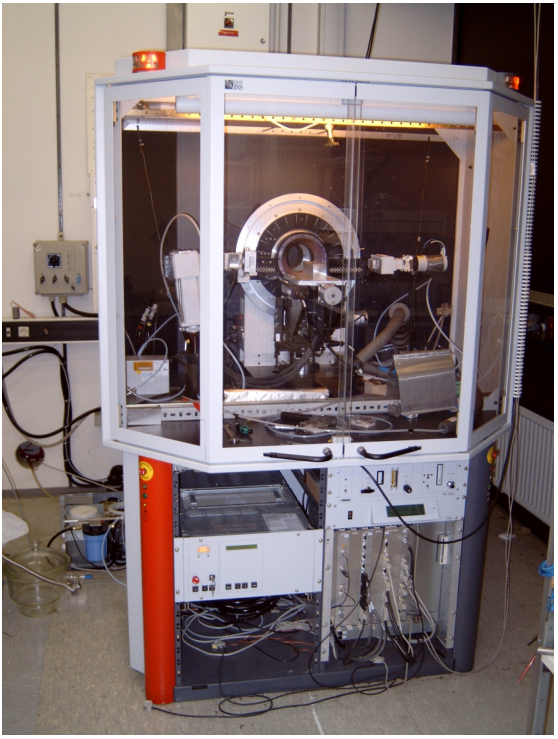
\includegraphics[width=0.4\textwidth]{bilder/apparatur.PNG}
  \caption{Das verwendete D8-Labordiffraktometers von der Firma Bruker AXS. \cite{sample}}
  \label{fig:app}
\end{figure}

Mit Hilfe des Gerätes kann sowohl der
Winkel der Röntgenröhre
als auch der Winkel des Detektors zum Probentisch
genau eingestellt werden. Desweiteren ist es
möglich den Probentisch in x-, y- und z-Richtung zu fahren.
Die Abbildung \ref{fig:anode_det} enthält zum Einen eine genaue Ansicht auf die
Röntgenröhre mit Blende und zum Anderen auf den Detektor des Gerätes.

\begin{figure}
  \centering
  \begin{subfigure}{0.59\textwidth}
  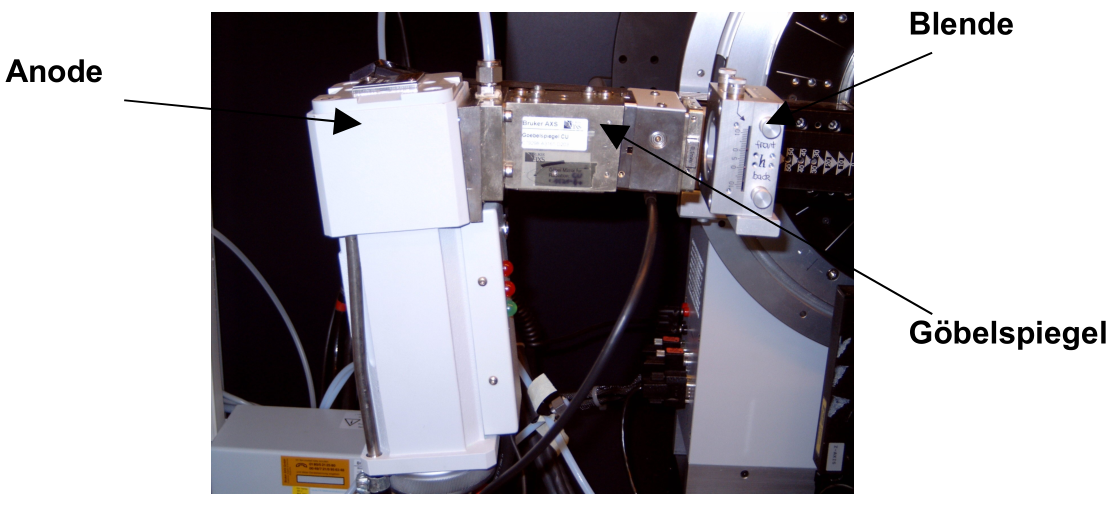
\includegraphics[height=3cm]{bilder/anode.PNG}
  \caption{Röntgenröhre mit Blende und Göbelspiegel.}
  \label{fig:anode}
\end{subfigure}
\begin{subfigure}{0.39\textwidth}
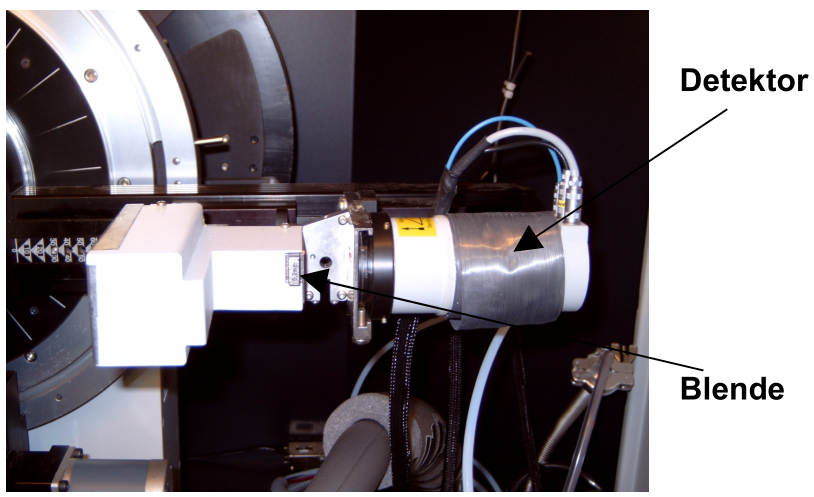
\includegraphics[height=3cm]{bilder/detektor.PNG}
\caption{Detektor mit Blende.}
\label{fig:det}
\end{subfigure}
\caption{Röntgenröhre \ref{fig:anode} und Detektor \ref{fig:det} des D8-Labordiffraktometers. \cite{sample}}
\label{fig:anode_det}
\end{figure}

Die Röntgenröhre besitzt eine Kupferanode und wird mit einer Spannung von $\SI{40}{\kilo\volt}$
und einem Strom von $\SI{40}{\milli\ampere}$ betrieben.
Die Röntgenstrahlen der Röntgenröhre werden durch den Göbelspiegel
gebündelt und monochromatisiert,
so dass der austretende Strahl eine Wellenlänge von
$\lambda=\SI{1.54}{\angstrom}$ besitzt.


\subsection{Justage des D8-Labordiffraktiometers}
\label{subsec:justage}
Bevor mit der Messung gestartet wird, wird das D8-Labordiffraktiometer
justiert. Dabei wird zwischen unterschiedlichen Justageschritten unterschieden.
% ?? strom und spannung hochfahren ??
% haben wir ja gar nichts mit zu tun gehabt


% % Probe justieren
% \paragraph{Probe justieren}


% Detektorscan
\paragraph{Detektorscan}
Bevor Justageschritte mit Probe unternommen werden, wird eine Primärstrahljustierung
vorgenommen. Dabei werden Röntgenröhre und Detektor so zueinander eingestellt,
dass sie einen Winkel von $\SI{0}{\degree}$ einschließen. Weiterhin wird die
Probe aus dem Strahlengang gefahren.
Anschließend wird ein sogenannter Detektorscan durchgeführt.
Dabei wird die Position der Röhre nicht verändert, allerdings die des Detektors.
Letzterer wird durch eine Drehbewegung aufsteigend durch den Strahl bewegt. Der Scanbereich
verläuft von $\SI{-0.5}{\degree}$ bis $\SI{0.5}{\degree}$. Nachdem die Messung beendet ist,
wird das Maximum lokalisiert und ein weiterer Detektorscan in einer symmetrischen
Umgebung der Größe $\SI{0.4}{\degree}$ um das Maximum herum, durchgeführt.
Nach Ende der Messung werden der Wert des Maximums, sowie die Halbwertsbreite
des Peaks notiert.

%  Z-Scan #1
\paragraph{Erster Z-Scan}
Um die Probenjustage zu prüfen,
wird ein sogenannter Z-Scan durchgeführt.
Bei diesem wird die Probe entlang der Z-Achse verschoben,
sodass reguliert werden kann, wie stark die Probe den Strahlengang
abdeckt. Im idealen Fall, bei dem die Probe parallel zur Strahlachse
orientiert ist, wird die Hälfte der Strahlintensität abgedeckt.
Daher wird genau der z-Wert gemessen, bei dem die Intensität auf
die Hälfte abgefallen ist. Der gemessene Wert wird vom Programm automatisch
verwendet um die Motoren ensprechend anzusteuern.


% Rocking-Scan 0 grad
\paragraph{Erster Rockingscan}
Nachdem die Probe zuvor möglichst parallel zur Strahlachse ausgerichtet wurde,
wird ein Rockingscan durchgeführt. Bei diesem werden Röntgenröhre und
Detektor gemeinsam symmetrisch um die Probe gedreht. In diesem ersten
Rockingscan wird für den Winkel zwischen Röhre und Detektor ein Wert von
$2\Theta = \SI{0}{\degree}$ gewählt. Die Drehung erfolgt in einem Winkelbereich
zwischen $\SI{-1}{\degree}$ und $\SI{1}{\degree}$. Nach Beenden des Scans wird
das Maximum der sich ergebenden Kurve ausgemessen und durch das Programm direkt
an die Motoren zur Anpassung weitergegeben.


% Z-Scan #2
\paragraph{Zweiter Z-Scan}
Anschließend wird ein zweiter Z-Scan durchgeführt um zu gewährleisten, dass
nach Anpassung gemäß des Rockingscans, die Probe wieder parallel zur Strahlachse
ausgerichtet ist. Dieser und der vorherige Schritt werden so lange ausgeführt,
bis die Justage sich nicht mehr
verbessert.



% Rocking-Scan 0.3 grad
\paragraph{Zweiter Rockingscan}
Für eine genauere Probenjustage, wird ein weiterer Rockingscan mit
$2\Theta = \SI{0.3}{\degree}$ durchgeführt. Der Winkelbereich für die Drehung,
wird von $\SI{0.1}{\degree}$ bis $\SI{0.2}{\degree}$ gewählt.


% Z-Scan #3
\paragraph{Dritter Z-Scan}
Zur feineren Justage, wird ein dritter Z-Scan durchgeführt.
Dabei wird für den Winkel zwischen Röntgenröhre und Detektor ein Wert von
$2\Theta = \SI{0.3}{\degree}$ gewählt. Der Bereich für die z-Koordinate
ist $[\SI{-0.5}{\milli\meter}, \SI{0.5}{\milli\meter}]$.
Nach Abschluss der Messung wird wieder das Maximum gemessen und
die Motoren entprechend angesteuert, sodass die bestmögliche Höheneinstellung
der Probe erreicht ist.


% Rockingscan 1.0 grad
\paragraph{Dritter Rockingscan}
Abschließend wird ein Rockingscan mit einer Winkeleinstellung von
$2\Theta = \SI{1}{\degree}$ durchgeführt. Der Scanbereich wird zwischen den Werten
$\SI{0.45}{\degree}$ und $\SI{0.55}{\degree}$ gewählt. Die Wahl dieses Scanbereichs lässt sich dadurch begründen,
dass bei $0.5$ das Maximum prognostiziert wird. Nach Vollendung der Messung
werden die Motoren wieder entprechend ańgesteuert, sodass das Diffraktiometer
nun vollständig justiert ist.



\subsection{Messung}
\label{subsec:messung}
Nachdem das Diffraktiometer justiert ist, wird
die eigentliche Messung durchgeführt.
Neben der eigentlichen Messung wird auch ein diffuser Scan durchgefürt,
um Störsignale abzuziehen.

% Messung mit Probe
Bei den Messvorgängen, wird ein Reflektivitätsscan vorgenommen.
Dabei sind $\alpha_{\text{i}}$ und der Winkel zwischen Probe und Detektor
$\alpha_{\text{f}}$ identisch. Beim diffusen Scan hingegen,
ist der Winkel des Detektors $\alpha_{\text{f}}$ um
$\SI{0.1}{\degree}$ verschieden vom Einfallswinkel $\alpha_{\text{i}}$.
Im verwendeten Programm, das die Messeinstellungen verwaltet, wird
"Omega / 2Theta" ausgewählt und ein Intervall von $\SI{0}{\degree}$ bis
$\SI{5}{\degree}$ vermessen.
Für die Schrittweite wird $\SI{0.05}{\degree}$
gewählt. Für die Dauer wird jeweils $\SI{5}{\second}$ gewählt.



% % Messung "Untergrund"
% Um die störende Signale aus den später aufgenommenen Messdaten
% entfernen zu können, wird der durchgeführt.
% Diese kann bei der Auswertung von den eigentlichen Messdaten abgezogen werden,
% um möglichst nur Informationen über die Probe zu erhalten.
